%====================================================================
% INTRODUCTION
%====================================================================
\section{Introduction}
\label{sec:intro}
%
Software complexity on tiny embedded processors is increasing.
%
Software supports a diversity of peripheral devices, multiple distributed middleware services, dynamic code updates and concurrent applications in a resource constrained environment.
%
Operating systems (TinyOS~\cite{levis05t2}, SOS~\cite{ram05sos}), Virtual Machines (Mat\'e, Sun SPOTS) and Wireless Applications (Zigbee~\cite{zigbee}) are some of the complex software systems running on 8-bit microcontrollers.
%
Implementing embedded software modules is a challenge, as programmers are forced to deal with severe resource constraints and concurrency issues.
%
Furthermore, there is very limited debugging support on tiny embedded processors, leading to an abundance of programming errors.
%
In particular, corruption of memory due to lack of protection from buggy applications is a very serious problem.
%
The impact of these errors can be quite severe.
%



%
Architecture of tiny embedded processors is very simple.
%
The entire memory is accessible to all software modules running on the processor via a single address space.
%
Architecture features such as memory management units (MMU) and privileged-mode execution are common only in desktop/server class processors to isolate and protect data and code of one program from another.
%
An MMU provides virtual memory in addition to protection and requires lot of memory for storing page tables for address translations.
%
Embedded microcontroller designers face extreme pressure to minimize cost and area of a chip.
%
Sometimes, even 32-bit ARM processor cores are not equipped with MMUs to minimize system cost and power~\cite{arm7tdmi}.
%
Therefore, current MMU designs will continue to be absent from low-cost low-power micro-controllers.
%


Software-based Fault Isolation (SFI) (or  ``Sandboxing") is a class of techniques proposed by Wahbe et. all for memory protection within single address space in desktop microprocessors.
%
In SFI, the address space of a process is partitioned into contiguous segments and each segment is allocated to a software module.
%
Software modules are implemented with run-time checks that ensure that all memory accesses reside entirely within the segment allocated to it.
%
These run-time checks are introduced through rewrite of a compiled binary.
%
Our approach is motivated by SFI but it has fundamental differences due to the resource constraints of the tiny embedded processors.
%
\textit{First}, we do not partition the address space of the microcontroller, as the available memory on microcontrollers is severely limited.
%
For example, the ATMEGA128 AVR has only 4 KB of on-chip RAM.
%
In most systems~\cite{hill02micro} this is the total available memory.
%
Static partitioning would further limit the memory that is available to individual software components.
%
Instead we rely on a \textit{Memory Map}: a data structure that can efficiently record ownership and layout information of the entire address space.
%
\textit{Second}, we do not rewrite binary to introduce run-time checks.
%
We instead enhance the implementation of \texttt{store, call} and \texttt{return} instructions in the microcontroller to perform run-time checks in hardware.
%
This minimizes the performance overhead of performing run-time checks in software and also eliminates the binary rewrite step of SFI which can be quite error prone.


Our overall system can be viewed as a hardware/software co-design approach to memory protection.
%
Low cost architecture extensions and a software run-time library work together to isolate different software components running on an embedded processor.
%
Our system is entirely implementable in software albeit with a high performance overhead.
%
Simple enhancements to the microcontroller core enable us to perform critical operations in hardware, thereby improving performance significantly.


\subsection{System Overview}
%
An overview of our system highlighting all its components is shown in Figure~\ref{fig:sys_overview}.
%
The final firmware image is composed of multiple software modules that need to be protected from one another.
%
%The software components are installed in separate protection domains.
%
A cross domain linking mechanism (described in Section~\ref{sec:cross_domain_linking}) installs the software modules in separate protection domains.
%
The cross domain calls are redirected through a software jump table.
%
The redirection assists the processor in determining the identity of the currently active domain.
%
The Memory Map (described in Section~\ref{sec:memmap}) tracks layout and ownership information for the protected address space.
%
The firmware image interacting with the memory map and hardware enhanced run-time checkers is guaranteed to be memory safe.
%
The cost and performance analysis of our system is done in Section~\ref{sec:eval}.
%
We present related work in Section~\ref{sec:related} and concluding remarks in Section~\ref{sec:conclude}.
%
\begin{figure}[htbp]
   \centering
   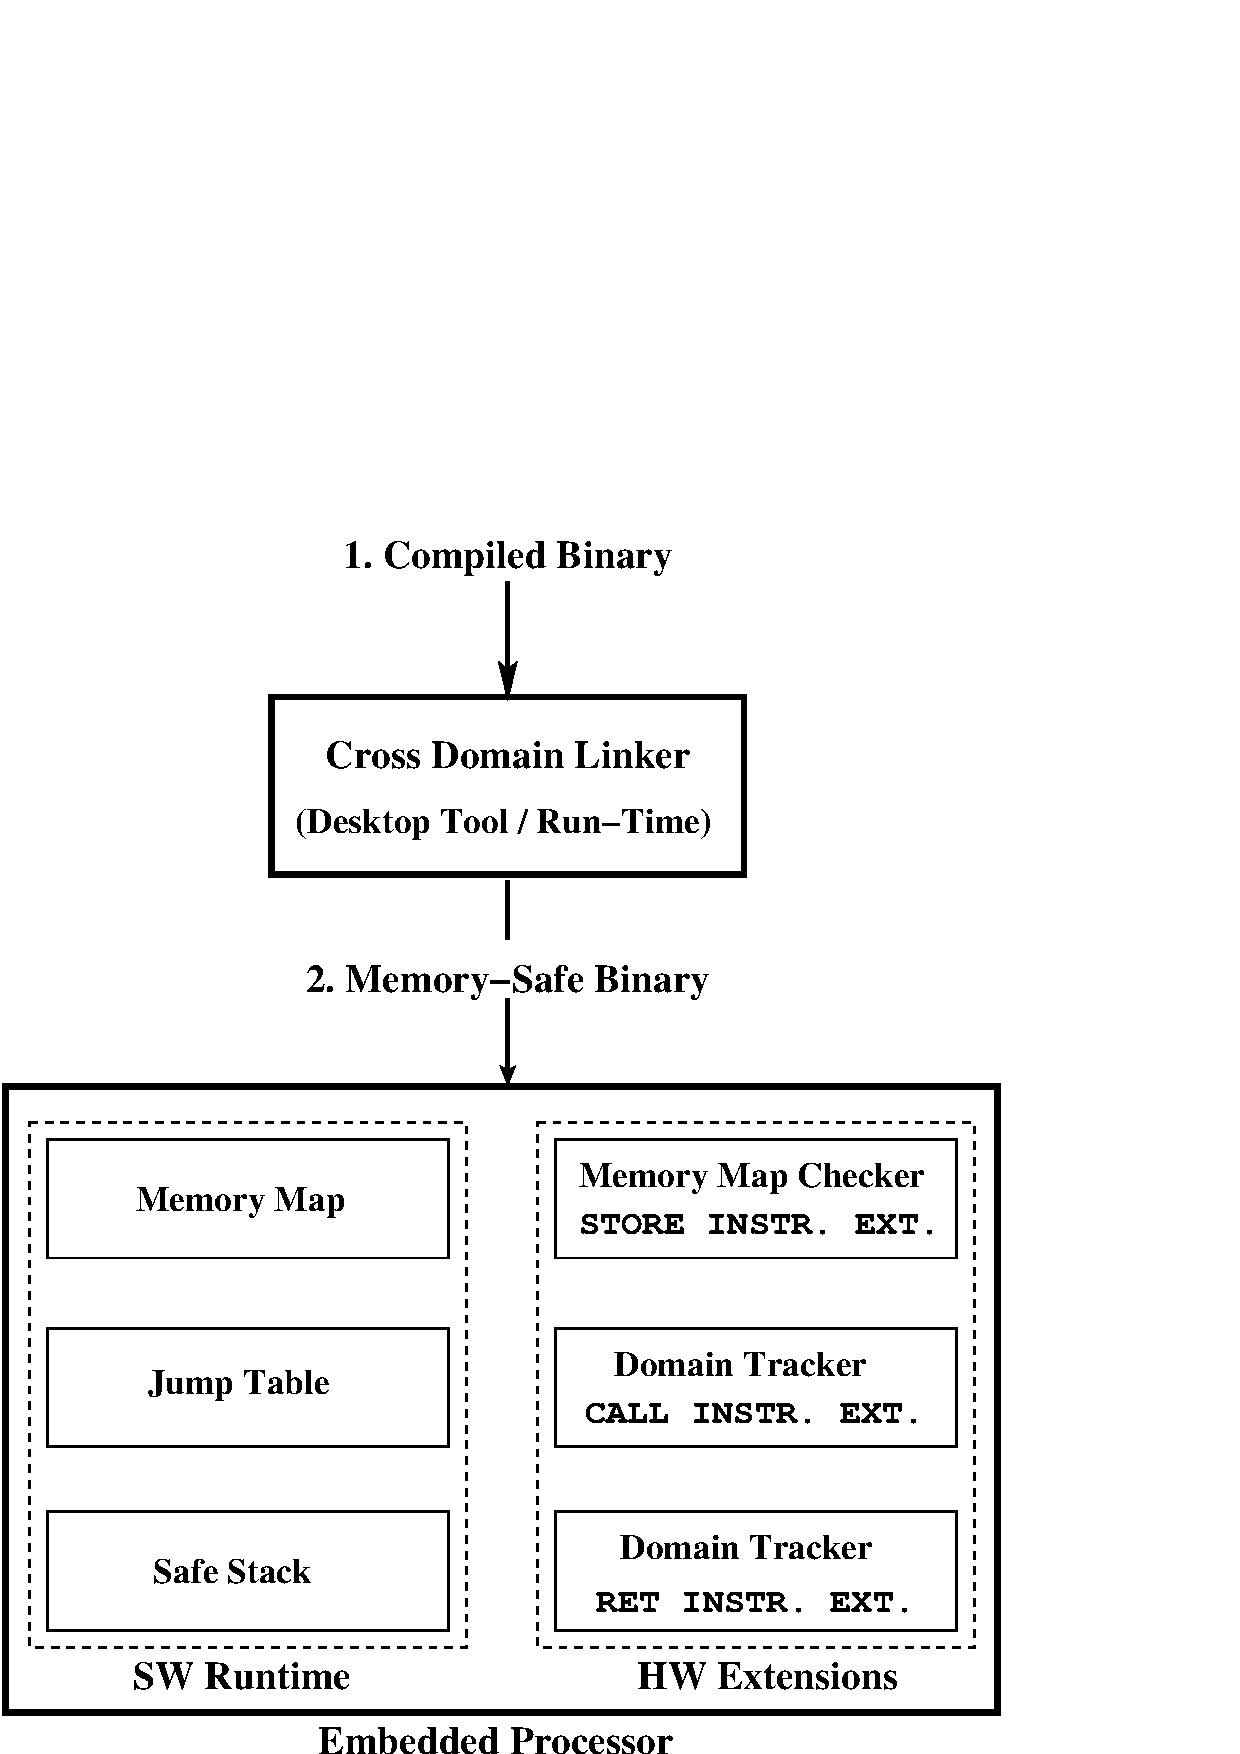
\includegraphics[height = 2.0in, keepaspectratio=true]{figures/sysoverview.pdf} 
   \caption{System Overview}
   \label{fig:sys_overview}
\end{figure}
%





